\documentclass[UTF8]{scrartcl}

\usepackage{xeCJK}
\usepackage{graphicx}
\usepackage{subfigure}
\usepackage{indentfirst}
\setlength{\parindent}{2em}

%opening
\title{HLS与Aladdin对比}
\author{}

\begin{document}

\maketitle

\begin{abstract}

\end{abstract}

\section{System Overview}
	
	HLS的典型流程如下图所示,在这一流程中HLS可以自动帮用户做的:1. 根据控制流生成合适的FSM结构; 2. 确定硬件资源; 3. schedule、资源分配; 4. 生成合适的中间表示。 需要用户来设置的:1. 并行度设置; 2. 模块之间如何交互; 3. 数据存储结构选择; 4. TIming Budget设置。 

	\begin{figure}[h]
 		\centering
		 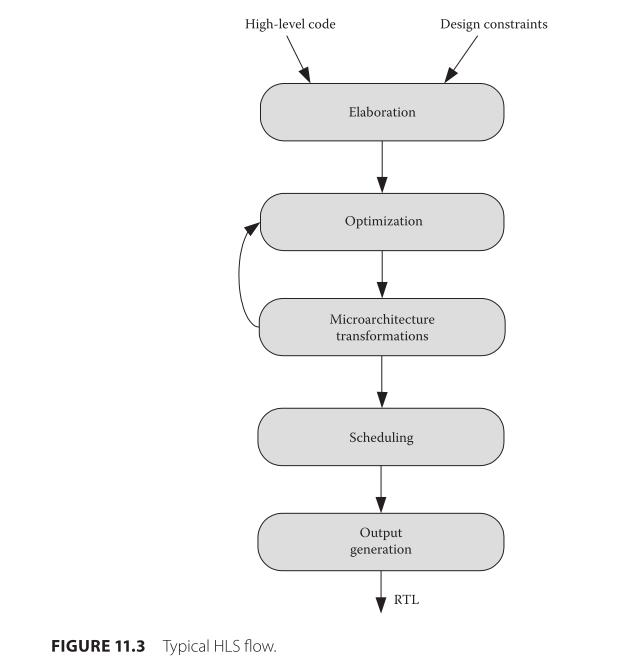
\includegraphics[width=3.50in,height=3.00in]{hls_flow.jpg} 
		\caption{HLS典型流程}
		\label{fig1}
	\end{figure}

\section{Input}

	Aladdin和HLS的输入都是高层语言的描述的算法和需要用户决定的硬件约束或选择。不同地方是HLS输入是高层语言的代码,而Aladdin输入的是代码运行的指令trace。原始代码包含更完整的逻辑结构而trace只包含执行的分支,但trace会包含执行过程中更多细节如实际的访存地址、寄存器分配等。

	\begin{table}[h]
		\centering
		\caption{Input对比}
		\begin{tabular*}{10cm}{c |c|c }
			\hline
			Input  &  HLS  & Aladdin   \\
			\hline
		     算法描述&High-Level code & C-code trace \\
			\hline
			 硬件约束&Hardware Constrain  &Hardware Config \\
			\hline
		\end{tabular*}	
	\end{table}
	
	
	
\section{Elaboration}
	第二步是要将输入的高层代码和硬件约束转化为可以做优化和处理的中间表示,一般基于图。HLS使用CDFG即control flow graph和data flow graph,前者表示控制逻辑后者表示计算,两者的联系是DFG中的节点对应CFG的一条边。而Aladdin使用data dependency graph,类似DFG,但因为输入是trace所以本身也体现了实际执行的控制流,没有再使用CFG,可以理解为为DFG映射到CFG的边中并根据实际执行结果展开后获得的graph。

		\begin{table}[h]
			\centering
			\caption{Elaboration对比}
			\begin{tabular*}{8cm}{c |c|c }
				\hline
				Elaboration  &  HLS  & Aladdin   \\
				\hline
				中间表示& CDFG & DDDG \\
				\hline
			\end{tabular*}	
		\end{table}
	
\section{Optimization}

	第三步是要对中间表示的graph做优化。在HLS中,DFG有两大部分的优化方法,其一来自于编译器如CSE等见图一,另一部分为硬件相关:
	
	\begin{itemize}
		
		\item[*] 位宽调整:根据数值的位宽或数值推断所需要的位宽。一般适用于Affine arithmetic,即与常数的乘加计算。在Aladdin中分析CNN一类应用时,位宽的调整来自于量化算法的分析。
		\item[*] Chain-to-Tree:时序相关,将链式转化为树型,例如加法链转化为加法器树,可以降低 latency。
		\item[*] Mux-Retiming:调整MUX与计算操作的位置,方便优化。
				
	\end{itemize}

	此外,还有针对CFG的优化方式,主要是准对条件判断(if,case)和循环(Loop)。 Aladdin中,由于trace中包含了访存等信息,优化主要体现在对Load/Store节点的处理。
	
			\begin{table}[h]
				\centering
				\caption{Optimization对比}
				\begin{tabular*}{16cm}{c |c|c }
					\hline
					Optimization  &  HLS  & Aladdin   \\
					\hline
					Compiler-related & Dead Code Elimination &  \\
					&Constant Folding and Propagation& \\
					&Common Subexpression Extraction&\\
					&Strength Reduction&\\
					&...&\\
					\hline
					Hardware-related&Bit trimming&Remove Repeated Load/Store\\
					&Chain-to-Tree&Store Buffer\\
					&Mux-retiming&\\
					&...&\\
					\hline
				\end{tabular*}	
			\end{table}

\section{Hardware Transformation}
	第四步则是将用户定义的硬件约束或设置在中间表达中实现,主要是对loop、function、array、pipeline等问题的处理。在这一阶段两者考虑的问题比较相似,但HLS具体的处理手段细节还不清楚。
	\subsection{Loop}
		Loop Unrolling,即通过将循环体复制多份从而展开了循环结构。完全展开和部分展开。Aladdin根据用户定义的unroll factor修改不同loop间的依赖关系,实现循环的展开。
		
		Loop Break:对于未展开的循环体中要执行的计算,其可能有多个cycle,如何插入合适的state将计算分配到不同的cycle。一般是自动的,Aladdin中根据定义的cycle time,当op的latency超过cycle time时即break。
		
		Loop Inversion:将while调整成do-whilt。
		
		Loop-invariant Code Motion:把循环中不变的操作移动到循环外。
		
		Loop Fusion:当两个循环迭代次数相同且没有数据依赖时,可以合并为同一个。
	\subsection{Functions}
		函数可以用来体现不同的硬件模块、相应的层次结构以及硬件资源的复用,但函数的使用不全是为了以上原因,使用inline函数则可以避免相应的优化。对于latency固定的函数,也可以做流水线的处理。 
		在Aladdin中每个节点的属性有函数这一项,可以用来实现复用等功能。
	\subsection{Array}
		Array在高层语言中用来表示数据,HLS和Aladdin对array的处理相似,主要有以下三种方式:
		使用Memory with read/write port实现,N latency。
		使用Register Bank实现,zero latency。
		Flatten array:将array展开为相互独立的变量。当array没有被flatten时,其访问会被看作单独的操作(graph中的节点),同时还要考虑访问同一地址时的冲突和数据依赖。
		Aladdin区分计算节点和访存节点,并根据不同存储的访存机制建立模型,包括仿真方式、latency和功耗等。
	\subsection{Pipeline}
		Loop pipeline只能应用于没有nested loops的循环,即需要将内层循环与外层merge才可以。Pipeline的变量包括stage(分为几级)、initial interval(每个stage耗用的周期数)和latency(执行完所有stage耗用的周期数)。scheduling pipeling即选择合适的stage nums并将loop内的操作分配至各个stage中,这个过程需要满足数据依赖的约束以及额外的pipeline约束。在HLS中,需要注意pipeline仍要保证原有的依赖关系。此外,还有不同loop之间的“loop-carried dependency”。而在Aladdin中,由trace可获得循环间数据的依赖关系,因此pipeline的实现主要通过修改不同的loop间的依赖关系
\section{Scheduling}
	在HLS中,schedule可以看作两个问题,1.将dfg中的操作map到cfg的边上(schedule );2.。 将dfg的操作map到对应的硬件资源中(binding)。优化的目标是latency或resources,由于有许多的可能情况,需要在设计空间中不断迭代(NP-complete)。 
	在Aladdin中,schedule的问题根据指令trace和数据依赖决定,不需要设置约束,而是由default的schedule规则,即依次将操作放入cycle中,当操作的总latency超过一个cycle时,则放入下一 个cycle; binding的规则是同一个function内乘法器复用加法器不复用,最终估算出需要的resource和latency,可以看做是HLS做探索时的一个情况。 
	
	在上述流程结束后,HLS可以生成对应的verilog代码(RTL),Aladdin则给出硬件执行的性能、功耗、面积等信息。

%\bibliographystyle{plain}

%\bibliography{refer}


\end{document}
